% Options for packages loaded elsewhere
\PassOptionsToPackage{unicode}{hyperref}
\PassOptionsToPackage{hyphens}{url}
\documentclass[
]{article}

\usepackage{xcolor}
\usepackage[margin=1in]{geometry}
\usepackage{amsmath,amssymb}
\setcounter{secnumdepth}{-\maxdimen} % remove section numbering
\usepackage{iftex}
\ifPDFTeX
  \usepackage[T1]{fontenc}
  \usepackage[utf8]{inputenc}
  \usepackage{textcomp} % provide euro and other symbols
\else % if luatex or xetex
  \usepackage{unicode-math} % this also loads fontspec
  \defaultfontfeatures{Scale=MatchLowercase}
  \defaultfontfeatures[\rmfamily]{Ligatures=TeX,Scale=1}
\fi
\usepackage{lmodern}
\ifPDFTeX\else
  % xetex/luatex font selection
\fi
% Use upquote if available, for straight quotes in verbatim environments
\IfFileExists{upquote.sty}{\usepackage{upquote}}{}
\IfFileExists{microtype.sty}{% use microtype if available
  \usepackage[]{microtype}
  \UseMicrotypeSet[protrusion]{basicmath} % disable protrusion for tt fonts
}{}
\usepackage{setspace}
\makeatletter
\@ifundefined{KOMAClassName}{% if non-KOMA class
  \IfFileExists{parskip.sty}{%
    \usepackage{parskip}
  }{% else
    \setlength{\parindent}{0pt}
    \setlength{\parskip}{6pt plus 2pt minus 1pt}}
}{% if KOMA class
  \KOMAoptions{parskip=half}}
\makeatother
\usepackage{graphicx}
\makeatletter
\newsavebox\pandoc@box
\newcommand*\pandocbounded[1]{% scales image to fit in text height/width
  \sbox\pandoc@box{#1}%
  \Gscale@div\@tempa{\textheight}{\dimexpr\ht\pandoc@box+\dp\pandoc@box\relax}%
  \Gscale@div\@tempb{\linewidth}{\wd\pandoc@box}%
  \ifdim\@tempb\p@<\@tempa\p@\let\@tempa\@tempb\fi% select the smaller of both
  \ifdim\@tempa\p@<\p@\scalebox{\@tempa}{\usebox\pandoc@box}%
  \else\usebox{\pandoc@box}%
  \fi%
}
% Set default figure placement to htbp
\def\fps@figure{htbp}
\makeatother
% definitions for citeproc citations
\NewDocumentCommand\citeproctext{}{}
\NewDocumentCommand\citeproc{mm}{%
  \begingroup\def\citeproctext{#2}\cite{#1}\endgroup}
\makeatletter
 % allow citations to break across lines
 \let\@cite@ofmt\@firstofone
 % avoid brackets around text for \cite:
 \def\@biblabel#1{}
 \def\@cite#1#2{{#1\if@tempswa , #2\fi}}
\makeatother
\newlength{\cslhangindent}
\setlength{\cslhangindent}{1.5em}
\newlength{\csllabelwidth}
\setlength{\csllabelwidth}{3em}
\newenvironment{CSLReferences}[2] % #1 hanging-indent, #2 entry-spacing
 {\begin{list}{}{%
  \setlength{\itemindent}{0pt}
  \setlength{\leftmargin}{0pt}
  \setlength{\parsep}{0pt}
  % turn on hanging indent if param 1 is 1
  \ifodd #1
   \setlength{\leftmargin}{\cslhangindent}
   \setlength{\itemindent}{-1\cslhangindent}
  \fi
  % set entry spacing
  \setlength{\itemsep}{#2\baselineskip}}}
 {\end{list}}
\usepackage{calc}
\newcommand{\CSLBlock}[1]{\hfill\break\parbox[t]{\linewidth}{\strut\ignorespaces#1\strut}}
\newcommand{\CSLLeftMargin}[1]{\parbox[t]{\csllabelwidth}{\strut#1\strut}}
\newcommand{\CSLRightInline}[1]{\parbox[t]{\linewidth - \csllabelwidth}{\strut#1\strut}}
\newcommand{\CSLIndent}[1]{\hspace{\cslhangindent}#1}
\setlength{\emergencystretch}{3em} % prevent overfull lines
\providecommand{\tightlist}{%
  \setlength{\itemsep}{0pt}\setlength{\parskip}{0pt}}
\usepackage[hang,flushmargin]{footmisc}
\usepackage{booktabs}
\usepackage{subcaption}
\usepackage{bookmark}
\IfFileExists{xurl.sty}{\usepackage{xurl}}{} % add URL line breaks if available
\urlstyle{same}
\hypersetup{
  hidelinks,
  pdfcreator={LaTeX via pandoc}}
\usepackage{ulem}
\usepackage{natbib}


\title{\textbf{How temperature regimes near the equinox synchronize spring biological events}\\[1em]}

\author{
Jonathan Auerbach\footnotemark[1]\\
\textit{Department of Statistics} \\ 
\textit{George Mason University}\\
\textit{Fairfax, VA USA}\\
\and
Andrew Gelman\footnotemark[2]\\
\textit{Department of Statistics} \\ 
\textit{Department of Political Science}\\
\textit{Columbia University} \\
\textit{New York, NY USA}\\
\and
E. M. Wolkovich\footnotemark[3]\\
\textit{Forest and Conservation Sciences} \\
\textit{University of British Columbia}\\
\textit{Vancouver, BC Canada} \\[1em]
}

\date{(Dated: April 26, 2026)}

\begin{document}

\twocolumn[
\maketitle

\begin{quote}
Many biological processes, including plant leafout and flowering, occur once cumulative temperatures reach a threshold (the thermal-sum model). In this way, temperatures are thought to coordinate the timing of biological events. Warming temperatures have thus also driven advances in spring events, especially leafout and flowering. But growing evidence suggests that with increasing climate warming, these advances have slowed (declining sensitivity) % JDMay10: something off about the tenses here... (DONE)
 and the variance in the timing of spring events has increased (declining synchrony)---raising questions about the resilience of temperature-based coordination to anthropogenic climate change. To answer these questions, researchers have complicated the thermal-sum model, introducing additional factors and mechanisms. We consider whether such complexity is necessary. Using results from the theory of stopped random walks, we show that sensitivity and synchrony are exactly as predicted by the basic thermal-sum model. The theory suggests a nonlinear relationship between temperatures and both the timing and synchrony of biological events. In particular, it predicts that as temperatures increase and springtime events shift from the equinox toward the winter solstice, % vvdm7May: I think I already told you, but I think this sentence can be confusing if you do not say explicitly: 'winter solstice' (DONE)
 the events themselves become less coordinated and more variable. We verify these predictions using experimental and real-world data, including 10,000 observations of common lilacs (United States, 1956-2025). We conclude that the theory provides a powerful tool for understanding the thermal-sum model---particularly when considering additional complexity. % JDMay10: this feels a little weak
\end{quote}

\vspace{2em}
]
{\renewcommand{\thefootnote}{\fnsymbol{footnote}}
\footnotetext[1]{jauerba@gmu.edu}
\footnotetext[2]{ag389@columbia.edu}
\footnotetext[3]{wolkovic@mail.ubc.ca}

\section{Introduction}\label{introduction}

Many biological events are triggered not by the temperature on a single day, but by the temperature accumulated over many days \citep{larcher1980}. A canonical example is the law of the flowering plants, % JDMay10:  is this really a 'law'?
which states that a bud blooms in the spring once cumulative temperatures exceed a plant-specific threshold. This and similar mechanisms are thought to synchronize a wide variety of seasonal events in an ecosystem---for instance, ensuring that pollinators emerge when flowers are in bloom. They also support an array of forecasting tools in which scientists track cumulative temperatures or `growing degree days' to predict harvest dates, manage pest emergence, and assess how shifting temperature patterns reshape ecological communities with climate change \citep{schwartzbook}.

Shifts in the timing of biological events have been the clearest fingerprint of anthropogenic climate change across both natural and managed systems \citep{ipcc2022}. But these shifts have proven difficult to fully predict or explain. The timing of phenological events have occurred earlier (i.e., advanced) as climates warm, however, the rate of advancement has slowed in recent years \citep{fu2015declining}.  At the same time, the variance in the timing of phenological events has in some cases declined and in others increased, without a clear pattern \citep{vitasse2018global,stemkovski2023disorder}. Higher variance has also manifested as previously unknown or rare phenological events becoming more common \citep{chuine2025living}. While research has provided myriad explanations---often with contrasting predictions and logic \citep{fu2015declining,wolkovich2021simple,gao2024thermal}---no work has examined the extent to which these observations are consistent with the basic thermal-sum model in which a biological event is triggered once cumulative temperatures reach a threshold. % JDMay10: TODO -- it feels that these observations are often interpreted as evidence the standard thermal sum model is wrong ...

Scientists have used the basic thermal-sum model for nearly two centuries \citep{quetelet1849letters}, but have rarely if ever integrated the relevant mathematical tools to characterize its behavior---% vvdm7May: 'developped': were the tools really developped specifically to characterize the behavior of the thermal-sum model? I wonder if you could just drop the 'developped' (DONE)
specifically results from renewal theory designed for analyzing stopped random walks. % vvdm7May: the last bit of this sentence ('specifically....') fall a bit "comme un cheveu sur la soupe" De you expect your readers to know about the renewal theory? AND % JDMay10:  I think you need to better explain how/why this theory is relevant to thermal sum models - including how we can consider an observed pheno event as being equivalent to the outcome of a stopped random walk.
Here we draw on these results to predict how events triggered by a cumulative temperature sum will shift with warming. Our model explains both the observed deceleration in the advancement of springtime events as well as the shifts in the variance. 

Throughout we emphasize the critical role of the temperature regime under which the biological events take place. For example, the variance in the timing of biological events can decrease or increase with warming depending on whether temperatures during the period of accumulation are stationary (as in the winter and summer near the solstice) or increasing (as in the spring near the equinox). We show that assuming the basic thermal sum model  % JDMay10:  edit made (DONE)
can (i) move spring events earlier at a faster or slower rate, and (ii) increase the variance of their timings, producing less synchronized events as they arrive earlier, a phenomenon we refer to as a `scattered spring.' 

\section{Results \& Discussion}\label{resultsdiscuss}
% JDMay10: can you add a sentence describing how this process could be modelled as a stopped random walk
Many springtime events occur when cumulative temperatures first reach or `hit' a plant-specific temperature threshold. We use results from renewal theory  \citep{siegmund1967some,  woodroofe1982nonlinear, gut2009stopped} to approximate the distribution of event times (hitting times) and thus predict the behavior of temperature-triggered biological events. % vvdm7May: Again, I wonder if you should explain a bit more, since the people in the ecology-related fields (such as me....) won't know about this renewal theory. Or at least add 'see Methods' or such?

Consider one such event, the bloom date of a bud. We model the effective temperature $X_i$---the daily temperature experienced by the bud on day $i$---in two temperature regimes, visualized in Figure 1. The first is the stationary temperature regime in which the average daily temperature $\alpha$ > 0 is constant. The stationary regime is commonly seen in the winter months following the solstice, and we refer to the temperatures in this regime as `winter temperatures.' The second regime is the increasing temperature regime in which the average daily temperature increases at constant rate $\beta$ > 0. The increasing temperature regime is commonly seen in the spring months closer to the equinox,  and we refer to it as `spring warming.' In both regimes, the effective temperature is the daily average temperature plus noise $\epsilon_i$. That is, $X_i = \alpha + \beta \, i +  \epsilon_i$ where $\beta = 0$ in the winter temperatures regime and $\beta > 0$ in the spring warming regime.

\begin{figure*}[t]
\centering
\pandocbounded{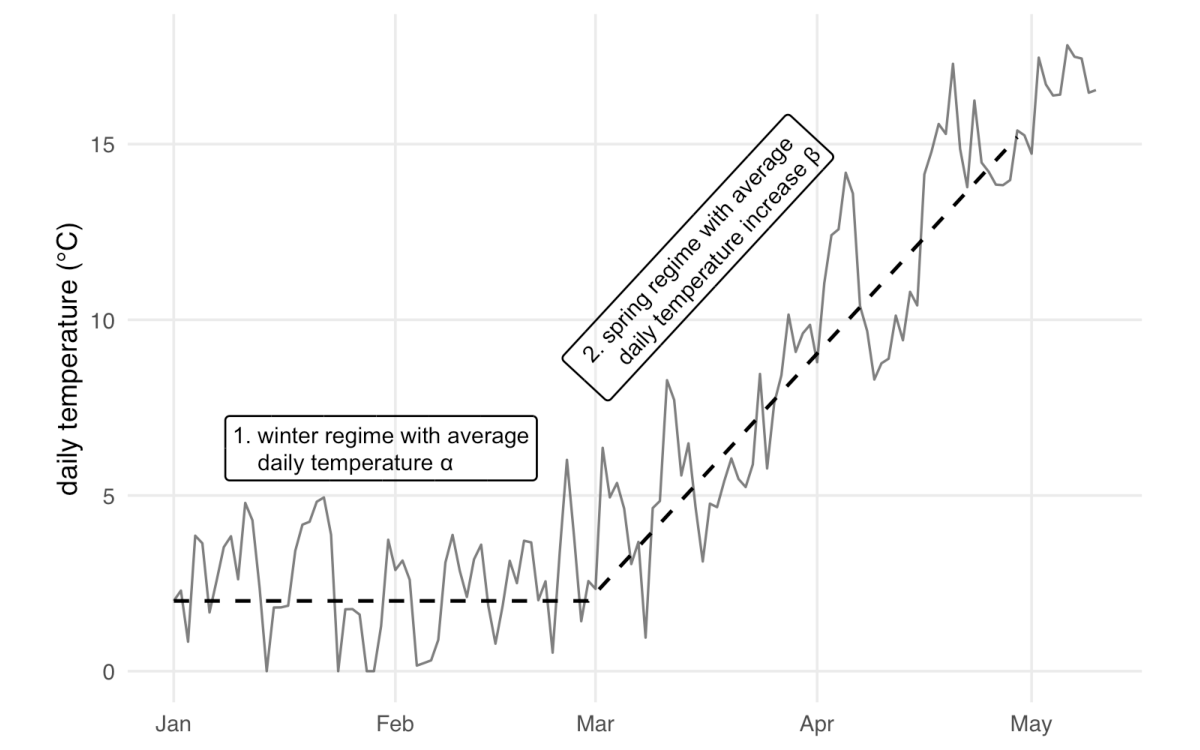
\includegraphics[keepaspectratio]{desynchronization_files/figure-latex/two_regimes-1.pdf}}
\caption{We model the daily temperature (solid line) as trend (dashed line) plus noise. 
The timing of springtime events in temperate climates depends on whether temperature is accumulated during one of two regimes, % JDMay10: presumably plants mix both regimes, with the time of transition being critical?
1. the stationary temperature regime (relatively flat near the winter solstice), which we refer to as `winter temperatures,' or 2. the increasing temperature regime (relatively linear near the spring equinox), which we refer to as `spring warming.'}
\end{figure*}
% vvdm7May: the question that comes to my mind looking  at this figure is: you're investigating \alpha, \beta, but can the transition timing from winter to spring also shift with ACC? Like, is the shift from stationary to non-stationary happen earlier (does the climatological spring happen earlier?)

Noise in this formulation could represent many biological factors depending on the scale and our developing understanding of what triggers springtime events. At the bud-level, it represents idiosyncratic variation at that bud, which could be driven by microclimate variation \citep{schwartz2014separating}, bud color variation \citep{peaucelle2022accurate}, or internal differences that vary when the bud starts accumulating temperatures \citep{vanderschoot2014, pan2023epigenetic}. We assume the $\epsilon_i$ are independent with mean $0$ and variance $\sigma^2$, although this assumption can be relaxed.

The bloom date $\nu(\tau)$ is the day $n$ that the cumulative temperatures $Z_n \;=\; \sum_{i=1}^n X_i$ first reach or `hit' % vvdm7May: you already said 'reach or hit' earlier, I think here you should choose one of the two
a plant-specific temperature-sum threshold $\tau > 0$, i.e. $\nu(\tau) \;=\; \min\{m:\, Z_m> \tau \}$. % vvdm7May: I would have used 'arg min' here? But I guess it's exactly the same meaning?
This formulation is common in growing degree day models, and more generally, $Z_n$ is the `forcing' part of most process-based models of plant phenology \citep{schwartzbook}. Standard results for stopped random walks yield asymptotic normal approximations for the bloom date \(\nu(\tau)\) when the thermal-sum threshold $\tau$ is sufficiently large that accumulation takes place over many days, as we would expect for most phenological thermal sums. % JDMay10: added edit (DONE) % vvdm7May: is 'many days' 2 weeks or 4 months? Maybe give an order of magnitude in parentheses? And do you need a reference for 'Standard results'?

These results predict that the mean and variance of bloom dates depend on the underlying temperature regime (i.e., values of \(\alpha\) and \(\beta\)) during which the plant accumulates temperature. In the winter temperatures regime, average temperatures are relatively % JDMay10: 'relatively' ? -- as in what do you mean 'by relatively flat?' I think
 flat during accumulation ($\beta = 0$), and cumulative temperature grows at an approximately linear rate. It follows that expected bloom date advances with climate change in step with increasing winter temperatures ($\mathbb{E}[\nu(\tau)] \approx \tau / \alpha$) as is often described in the literature \citep{vitasse2022great}. In the spring warming regime, average temperatures increase during accumulation ($\beta > 0$), and cumulative temperatures grow quadratically. In this regime, bloom date advances as a function of the rate of spring warming ($\mathbb{E}[\nu(\tau)] \approx \sqrt{ 2 \tau / \beta}$). 

Within either regime, the relationship between bloom dates and temperature is non-linear as observed in recent papers \citep{fu2015declining,wolkovich2021simple}. Increasing temperatures advance bloom dates at a diminishing rate as warming % vvdm7May: maybe you could explicitly say 'sensitivity' here, since you mention this term in the abstract
(measured by the winter temperatures $\alpha$ or spring warming $\beta$) increases (for the winter temperatures regime: $\frac{\partial}{\partial \alpha}\,\mathbb{E}[\nu(\tau)] \approx - \tau / \alpha^2$; for the spring warming regime: $\frac{\partial}{\partial \beta}\,\mathbb{E}[\nu(\tau)] \approx -\frac{1}{2}\sqrt{ 2\tau / \beta^{3}}$). But when climate change shifts the period when plants accumulate temperatures from the spring warming regime to the winter temperatures regime, % JDMay10:  aren't you shifting from the winter to the spring warming earlier?
advances may accelerate, % vvdm7May: is this something that is sometimes observed? % JDMay10:  small edit made (DONE)
particularly if increases in winter temperatures $\alpha$ outpace increases in spring warming $\beta$. . % vvdm7May: outpace how much? How do you quantify 'outpace'? Since alpha and beta are not in the same units, I guess it depends on the duration of the spring? Was this kind of acceleration observed in the field? I.e. an increasing sensitivity after a declining sensitivity? If never observed, why? Maybe just not yet? Do you have such cases in your lilac observations where the sensitivity is increasing? I feel there is something really nice to dig up here, as with your nice simple approach you might be abble to make predictions with further warming? I could even see a figure where we see the sensitivity decreasing and then increasing at some point where the event happens during the winter and not in the spring anymore! "Not only we explain why the sensitivity has declined in the last decade, but also we predict that the decline will turn back..." or some similar idea to discuss (if it's true)

Importantly, the effects of warming within the two regimes % JDMay10: edit made
make very different predictions regarding the synchrony of events---that is the variance in event timings within the same year and location. Both predict decreased variance with warming (for the winter temperatures regime: $\mathrm{Var}(\nu(\tau)) \approx \sigma^2 \, \tau / \alpha^3$; for the spring warming regime: $\mathrm{Var}(\nu(\tau)) \approx \sigma^2 / \sqrt{2 \beta^{3} \tau}$), but the influence of noise % JDMay10:  can you call this something else, perhaps 'sensitivity to independently fluctuating variables (here represented by our noise parameter) '
is strikingly different as reflected by whether the threshold $\tau$ is in the numerator or the denominator. % vvdm7May: I feel the end ofr this sentence could be confusing for some readers, as you mention 'noise' but then go straight to \tau. Maybe you just need to say explcitly to say that 'noise \epsilon' is buffered or amplify depending on the position of '\tau' or something similar...? 

% JDMay10: couple small edits made below and next paragraph (DONE)
In the spring warming regime, the threshold $\tau$ is in the denominator, and thus the variance is small when the threshold is large---reflecting the fact that noise is quickly overwhelmed by the quadratic increase in cumulative temperatures that occurs during spring warming. This effectively acts to synchronize plants (and buds within plants) with the same threshold---making idiosyncratic differences such as microclimate negligible. In contrast, under the winter temperatures regime, the threshold $\tau$ is in the numerator, and thus the variance is large when the threshold is large. Thus noise can remain relatively influential so that idiosyncratic differences translate into larger differences in threshold-crossing times. % vvdm7May: in the winter regime, the variance is large when \tau is large, but with a larger \tau you're more likely to fall in the spring regime right?

The fact that the variance is predicted to be small in the spring warming regime and larger in the winter temperatures regime suggests that the observed variance will increase when anthropogenic warming shifts accumulation from the spring warming regime to the winter temperatures regime. % JDMay10: this feels backwards to me, but perhaps spring warming does not come earlier with climate change?
The shift in regimes is observable in phenology as a `scattered spring' in which springtime events simultaneously advance and become less coordinated.

% vvdm7May: smoother transition?
Not all warming scatters spring. Whether warming leads to a more synchronized or more scattered spring depends on the local joint evolution of % JDMay10: can we change 'local joint evolution of' to 'transition between'?
winter temperatures and spring warming ($\alpha$ and $\beta$) and on the threshold ($\tau$) relevant for a given species and life-cycle event. 
In some locations, climate change may manifest primarily as higher winter temperatures (an increase in \(\alpha\)) with relatively little change in the rate at which temperatures rise during spring (a modest change in spring warming \(\beta\)). In others, winter temperatures may change less while spring transitions steepen (a larger increase in spring warming \(\beta\)). % JDMay10:  I was imagining a scenario where spring non-stationarity occurs earlier ...

% JDMay10: I think you need to just formally introduce this 'framework' (stopped-random-walk framework) above, at start of the section
The stopped-random-walk framework offers a simple way to translate this spatially varying climate change into spatially varying predictions % vvdm7May: but you miss the opportunity to axcutally show these spatial predictions! Figure 2 is still quite theoretical, and it's not that clear that you use actual observations! 
of both the advancement of spring and its variability. To demonstrate the framework, we model bloom dates from the lilac--honeysuckle phenology network compiled by \cite{rosemartin2015lilac}, collected across the continental United States from 1956--2014. We limit our analysis to the purple common lilac (\textit{Syringa vulgaris}) and the phenophase full bloom, and we update the dataset using USA National Phenology Network records from the same sites and species until 2025 \citep{switzer_etall:2025}.

\begin{figure*}
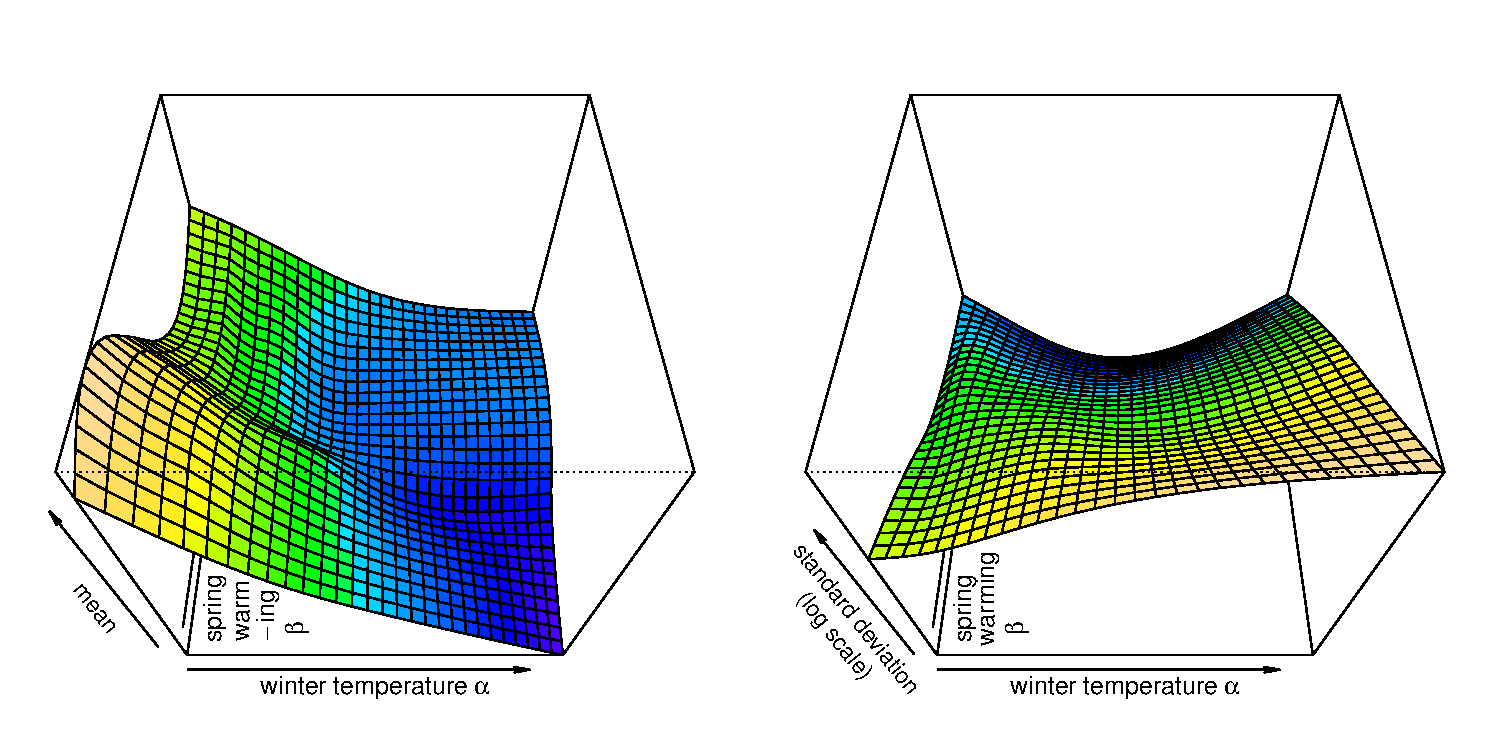
\includegraphics[width=1\linewidth]{desynchronization_files/figure-latex/lilac_te_mean-1} \caption{Mean and log standard deviation of lilac bloom dates (n = 10,613 from Rosemartin et al. 2015, updated to 2025 using USA National Phenology Network data) by winter temperatures $\alpha$ and spring warming $\beta$ as estimated by a generalized additive model. The mean (left) decreases as $\alpha$ and $\beta$ increase. The standard deviation (right) can increase or decrease depending on the relative values of $\alpha$ and $\beta$.} % vvdm7May: 'trends' rather than 'values'?
\label{fig:lilac_te_mean1} % vvdm7May: where is the color scale legend? You have interpretable units (days), so it would be nice... And maybe you need unit on your axis?!
\end{figure*}
% vvdm7May: with the abstract, I would kind of expect two panels: 'Sensitivity', and 'Synchrony'. The right panel is already about synchrony, but maybe the left panel could be transform to 'sensitivity' (to warming). Or add a third panel if you want to keep the mean? I don't know if it's clear

\begin{figure*}
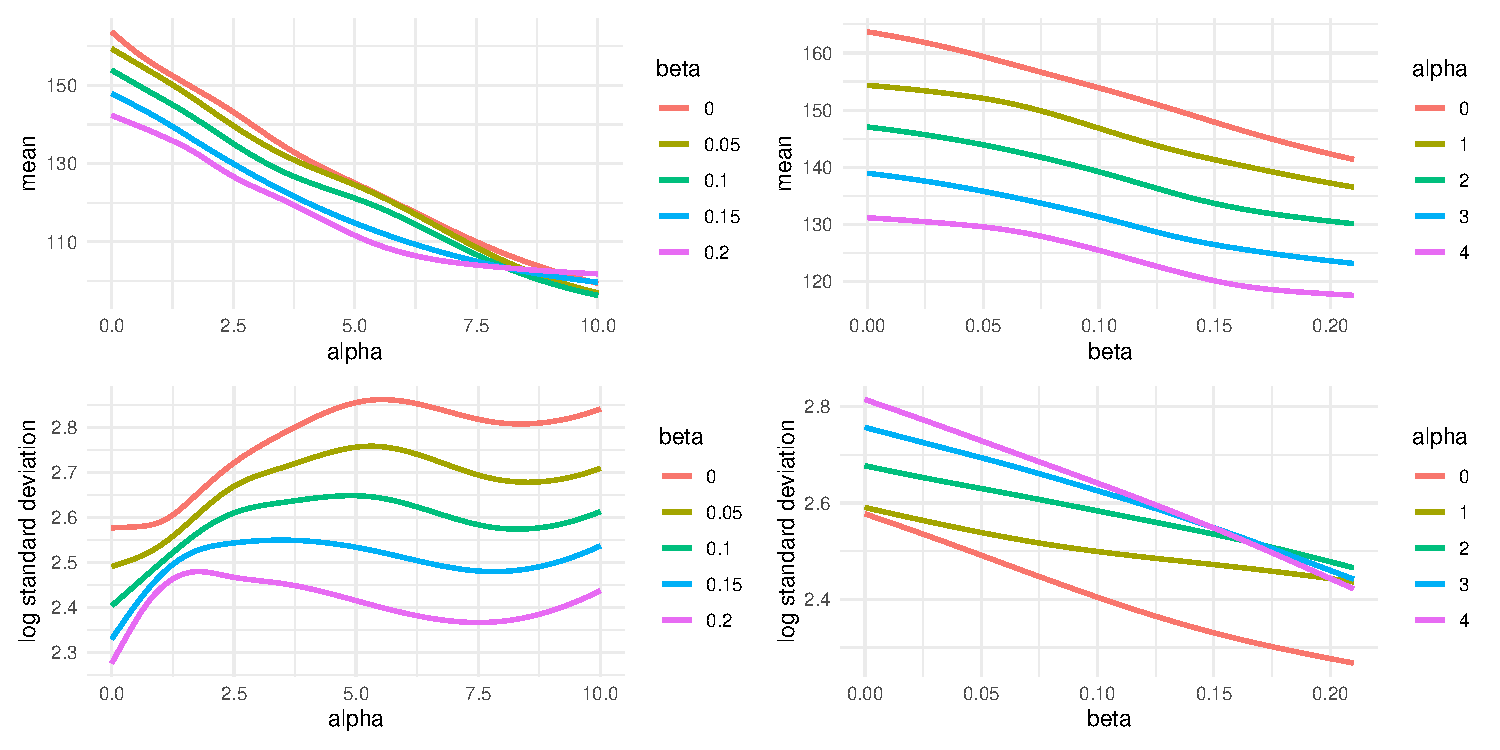
\includegraphics[width=1\linewidth]{desynchronization_files/figure-latex/lilac_te_mean-2} \caption{Mean (top) and log standard deviation (bottom) of lilac bloom dates (n = 10,613 from Rosemartin et al. 2015, updated to 2025 using USA NPN records) by winter temperatures $\alpha$ and spring warming $\beta$ as estimated by a generalized additive model. The top two figures show the mean generally decreases as \(\alpha\) increases holding \(\beta\) constant (left) and \(\beta\)  increases holding \(\alpha\) constant (right). The bottom two figures show the standard deviation can increase or decrease depending on whether \(\alpha\) increases with \(\beta\) held constant (left) or \(\beta\) increases with \(\alpha\) held constant (right).} % vvdm7May: Here you're using the same color palette as in Figure 2 but for a different meanig, that could be confusing.... maybe...
% And you might also want to add the units on the axis? You have interpretable parameters with real units, you should be proud!
\label{fig:lilac_te_mean2}
\end{figure*}

For each record, we estimate winter temperatures $\alpha$ and spring warming $\beta$. We then estimate the conditional mean and log standard deviation functions of the bloom date given $\alpha$ and $\beta$  using a generalized additive model \citep{hastie1986generalized, wood2017generalized}. The two functions are displayed in Figure \ref{fig:lilac_te_mean1}. Select cross sections of these functions are displayed in Figure \ref{fig:lilac_te_mean2}. Note that the bloom date is measured in days since January 1 of the observation year.

These two figures show that increasing either winter temperatures $\alpha$, spring warming $\beta$, or both shift flowering times exactly as predicted by the theory. % JDMay10: what theory?
Increasing $\alpha$ or $\beta$ is associated with earlier mean bloom dates, which generally but not always advance at a decreasing rate. % vvdm7May: again, explicit mention to 'sensitivity'?

% JDMay10: wanted us to get rid of 'associated with' below a few places and swap () stuff (DONE)
Increasing $\alpha$ and holding $\beta$ fixed returns greater variance (higher log standard deviation), while increasing $\beta$ while holding $\alpha$ fixed returns lower variance (lower log standard deviation). This is the `scattered spring' predicted from the theory: When $\beta$ is fixed, increasing $\alpha$ means more buds bloom in the winter temperatures regime, under which conditions the variance is predicted to be larger. When $\alpha$ is fixed and $\beta$ is increased, the percentage of buds blooming in either regime does not change. % vvdm7May: the percentage does nto change only if the timing of the transition between winter and spring is fixed (see my comment on figure 1)
Rather the fixed percentage of buds that bloom under spring warming are subject to increased warming, and under these conditions the variance is predicted to be smaller.  % vvdm7May: what is the relative importance of increasing Var under increasing alpha vs. decreasing Var under increasing beta? Similar in amplitude? Or increase/decrease more important?

 % vvdm7May: You're missing a transition! I think you should explain why you complement your analysis on observational data with experimental stuff. A simple justification can be what you explain later, that is "factors like chilling and photoperiod, as these are held fixed"
% JDMay10:  need to explain why you do this also, what does this allow us to learn that we could not learn from the lilacs?
We also apply the framework to experimental data from \cite{Charrier:2011aa} in which stems were sampled from 30 walnut trees (\textit{Juglans}\textasciitilde sp.) trees, chilled at \(4^\circ\)C, % vvdm7May: who cares about the exact chilling treatment?
and then warmed at various constant temperatures until budburst.

Since temperatures are held constant, this experiment replicates the winter temperatures regime in which the bloom date is approximately normal with mean $\tau / \alpha$ and variance $\sigma^2\,\tau / \alpha^3$, which we fit using weighted least squares. Figure \ref{fig:experiment} shows the observed data (points), model fit (solid line), 95\% confidence interval (inner grey region, approximately two standard errors), and 95\% prediction interval (outer grey region, approximately two standard deviations). % vvdm7May: I would put the 'Figure ... shows...' sentence in the caption
The data fit the model well, exhibiting the nonlinear relationship in the mean and variance as predicted by the theory, as we describe above. The relationship cannot be explained by factors like chilling and photoperiod, as these are held fixed. % JDMay10: Need to indicate that nonlinearity has previously been ascribed to chilling and photo, so you also fit the model to experimental data on walnut trees where chill and photo have been held constant.

\begin{figure*}[t]
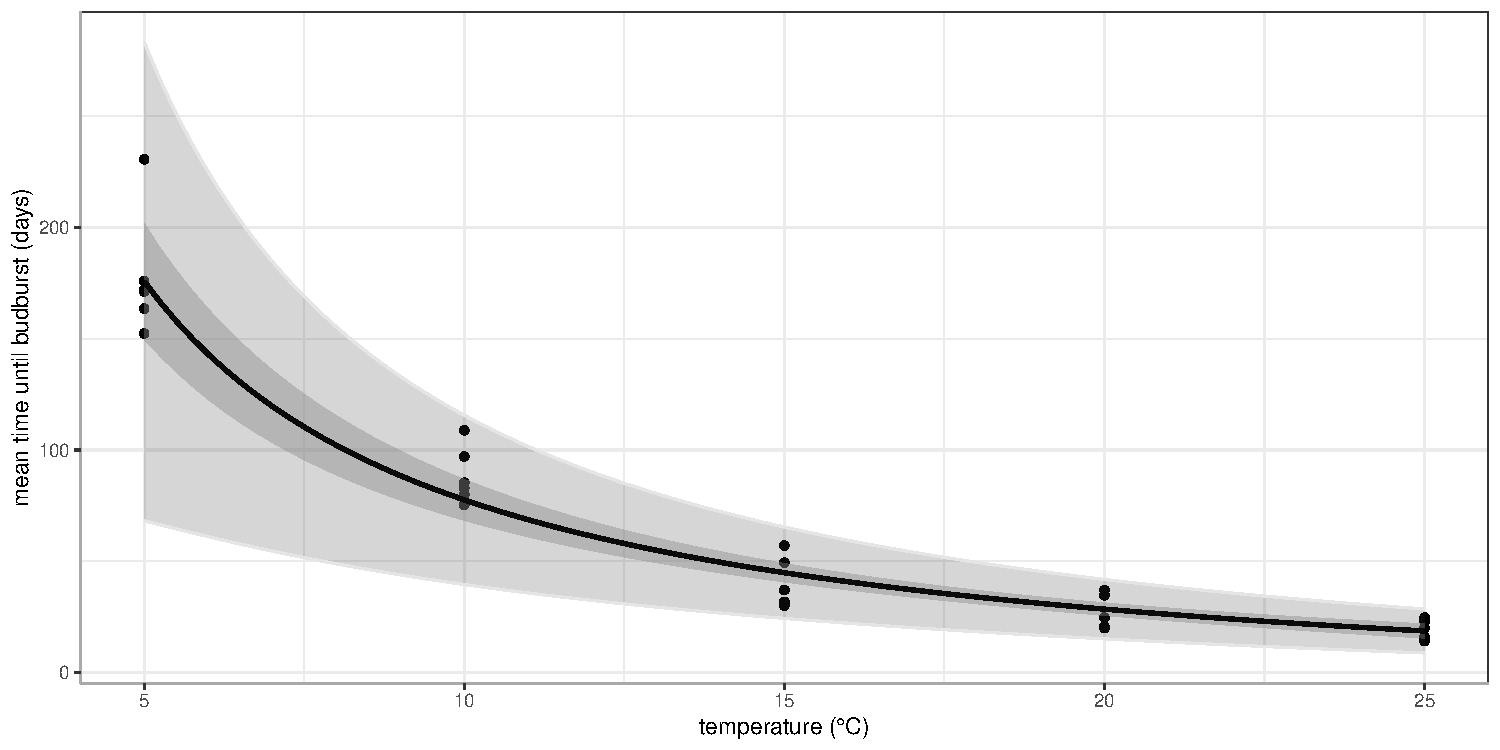
\includegraphics[width=1\linewidth]{desynchronization_files/figure-latex/experiment} \caption{Mean time until budburst as a function of the average daily temperature in a controlled experiment conducted by Charrier et al. (2011) in which stems were sampled from 30 walnut trees (\textit{Juglans}\textasciitilde sp.) trees, chilled at \(4^\circ\)C, and then warmed in different environments (x-axis) until budburst. Constant warming reflects the winter temperatures regime. Conditional mean (solid line) estimated using weighted least squares. Inner interval represents the confidence interval (approximately twice the standard error) while the outer interval represents the prediction interval (approximately twice the standard deviation). The figure shows that the mean and variance are nonlinear even when chilling and photoperiod are held fixed. Both decrease with increasing temperatures as predicted by the thermal-sum model.} % vvdm7May: I feel you might want to say explicitly that the x axis shows an icnreasing \alpha or winter 
\label{fig:experiment}
\end{figure*}

% JDMay10: need to explain why you did this (or just cut it!). ... and some small edits
As a check, we also conduct both analyses using an alternative approach in which we bin the data by quartile of $\alpha$ and $\beta$, and we reach similar conclusions. See Appendix for details. We conclude that the basic thermal-sum model is sufficient to explain the observed shifts in springtime events. In particular, it explains why warming is associated with both decelerating advances % vvdm7May: and not yet accelerating advances..?
and either increasing or decreasing variances \citep{vitasse2018global, fu2015declining, stemkovski2023disorder}. We stress that this framework makes minimal biological assumptions, only that the events are triggered by a thermal-sum, the same assumption made by most growing degree day or spring forcing models \citep{schwartzbook}. % JDMay10:  'We suggest alternative models that require fitting additional parameters should first be compared with this simpler ... (also suggests merge to next pargaraph)
The model does not preclude complicated explanations. However, given the fact that the thermal-sum model is parsimonious and nearly two centuries old \citep{quetelet1849letters}, the burden falls on complicated models to justify their complexity. For example, winter chilling and photoperiod are often invoked to explain the observed shifts in springtime events \citep{fu2015declining}. These factors are already implicitly accounted for in the thermal-sum model, which allows for idiosyncratic variation. % vvdm7May: maybe explicitate a bit more what you mean exactly?
Our results question whether explicitly modeling these factors is necessary and thus justified. % JDMay10: I am not convinced by this argument, if they are in the 'noise parameter' don't we want to reduce noise, improve our mechanistic understanding, and have better predictions? A separate question is whether we *need* to include them in models given our specific goals.



More generally, the theory % JDMay10: what theory? the thermal sum model is the theory, right? I think you show how we can better understand predictions of this model
presented provides opportunities for new experiments and observational insights on which the basic thermal-sum model may be improved. As it stands, % JDMay10: not clear - are you suggesting this from your interpretation of the thermal sum model (assuming a stopped random walk) or this the expectation from previous interrogation of this (thermal sum) model? If the latter, what new insight has your provided.
the basic thermal-sum model predicts a general desynchronization of spring events as their timing moves closer to the solstice. Absent some compensating mechanism, the timing of biological events across the ecosystem---from crops to forests, and from plants to insects---will in many cases become more variable, with potential cascading consequences for industry and natural ecosystems.


\subsection{Methods}\label{methods}

% JDMay10: better define GHCND (DONE) and day index (not done) 
Our observational data analysis considers all sites in the historical lilac--honeysuckle phenology network \citep{rosemartin2015lilac} that recorded the phenophase full bloom and were within 10 miles of a Global Historical Climatology Network daily (GHCNd)  site with sufficiently complete temperature records. We limit our analysis to common lilac (\textit{Syringa vulgaris}). We include all observations made from 1955 to 2025 as recorded by the USA National Phenology Network, retrieved using the \texttt{R} package \texttt{rnpn}, resulting in \(10,613\) observations. 

For each observation, we estimate \(\alpha\) using the average daily temperature between January and February. We estimate \(\beta\) using the slope of a linear regression model fit by regressing daily temperature on day index over March and April. Temperatures below \(0\) are set to \(0\), a common base temperature in growing degree day models. 

% vvdm7May: Figure 4 seems to be results with Charrier data 
The parameters \(\alpha\) and \(\beta\) are shown for nine sites in Figures 5-7 in Appendix A.3. Figure 5 shows nine randomly selected site-years and has the same interpretation as Figure 1. Site 14726 in New Mexico (Year 1969) is a good example of a bloom in the spring warming regime since relatively little temperature was accumulated during January and February. The average bloom date was May 8th with a standard deviation of 17 days. Site 14276 in New York (Year 1982) is a good example of a bloom between the winter temperatures and spring warming regimes, which had an average bloom date of March 18 with a standard deviation of 27. Figures 6 and 7 show \(\alpha\) and \(\beta\) for the nine sites with the longest running records.

We fit a two-parameter Gaussian location--scale model using the \texttt{gaulss} function from the \texttt{R} package \texttt{mgcv} in which we define 
\begin{align*}
 \mu(\alpha,\beta)&=\mathbb{E}[\nu(\tau) \mid \alpha,\beta] \\[1em]
 \sigma(\alpha,\beta)&=\mathrm{SD}(\nu(\tau) \mid \alpha,\beta).
 \end{align*} 
 Both \(\mu\) and \(\sigma\) are modeled with tensor-product splines with basis dimension k = 10. The fitted functions are shown in Figures \ref{fig:lilac_te_mean1} and \ref{fig:lilac_te_mean2}.

\bibliographystyle{apalike}
\bibliography{desynchronization}

\onecolumn

\section{A. Appendix}\label{a.-appendix}

\subsection{A.1 Sketch of Theoretical
Results}\label{a.1-sketch-of-theoretical-results}

We follow the notation in \cite{gut2009stopped}. Let
\(X_i=\alpha+\beta i + \epsilon_i\) denote the temperature on day \(i\),
where \(\alpha>0\), \(\beta\ge 0\), and the \( \{\epsilon_i\} \) are 
independent and identically distributed with  
\(\mathbb{E}[\epsilon_i]=0\) and 
\(\mathrm{Var}(\epsilon_i)=\sigma^2\). Define the deterministic
cumulative sum \[
\xi_n=\sum_{i=1}^n \mathbb{E}[X_i]
=
\alpha n+\frac{\beta}{2}n(n+1)
=
\frac{\beta}{2}n^2+\beta\gamma n,\]
where \(\gamma=\frac{\alpha}{\beta}+\frac{1}{2}\)
and \(\xi_n=\alpha n\) when \(\beta=0\). 

Denote the sum of the
stochastic component \(S_n=\sum_{i=1}^n \epsilon_i\). The object of
interest is the first-passage time of \( Z_n=S_n+\xi_n\), \[
\nu(\tau)=\min\{n\ge 1:\ Z_n> \tau\}.
\] 

In the language of \cite{lai1977nonlinear}, \(\{Z_n\}\) is a
perturbed random walk. That is, the random walk \(\{S_n\}\) is perturbed by the
deterministic term \(\{\xi_n\}\). This setup yields two
asymptotic regimes, corresponding to the empirical distinction between
the winter temperatures regime in which \(\beta\approx 0\) and the spring warming regime in which \(\beta>0\).

When \(\beta=0\), we apply the usual asymptotic argument for
the hiting time of a random walk with constant positive drift as \(\tau \to \infty\), \[
\nu(\tau)\ \dot{\sim}\ \mathrm{Normal}\!\left(\frac{\tau}{\alpha},\ \frac{\sigma^2\,\tau}{\alpha^{3}}\right),
\] see \cite{gut2009stopped}.

When \(\beta>0\), the deterministic component
\(\xi_n=\frac{\beta}{2}n^2+\beta\gamma n\) grows quadratically so that
the threshold \(\tau\) is reached near the deterministic crossing time
\(m(\tau)\) satisfying \(\xi_{m(\tau)}\approx \tau\). The solution is \[
m(\tau)=\frac{-\beta\gamma+\sqrt{\beta^2\gamma^2+2\beta \tau}}{\beta}
=
\sqrt{\frac{2\tau}{\beta}}-\gamma+o(1).
\] By the functional central limit theorem, the deviation of \(\nu(\tau)\)
about \(m(\tau)\) is approximately normal. Linearization of
\(Z_{\nu(\tau)}\approx \tau\) around \(m(\tau)\) yields \[
\nu(\tau)\ \dot{\sim}\ \mathrm{Normal}\!\left(m(\tau),\ \frac{\sigma^2\,m(\tau)}{\bigl(\alpha+\beta\,m(\tau)\bigr)^2}\right)
\;\approx\;
\mathrm{Normal}\!\left(\sqrt{\frac{2t}{\beta}}-\gamma,\ \frac{\sigma^2}{\beta^{3/2}\sqrt{2t}}\right),
\] where we have used the fact that
\(\alpha+\beta m(\tau) \approx \beta m(\tau) \approx \sqrt{2\beta \tau}\) when
\(\tau\) is large. 

It follows that in the spring warming regime, the mean hitting time scales like
\(\sqrt{\tau}\) (rather than linearly in \(\tau\) as in the winter temperatures regime) and the variance shrinks at
rate \(\tau^{-1/2}\) (rather than growing at \(\tau\) as in the winter temperatures regime).


\subsection{A.2 Additional Tables}\label{a.2-additional-tables}

In addition to the model-based approach in the main text, we also examine the data using a binning approach. 
The results are contained in Tables  \ref{tab:walnut_forcing}-\ref{tab:sd_bloom_bins}.

\begin{table*}[t]
\centering
\caption{Summary data from the Walnut forcing experiment (Charrier et al. 2011).}
\label{tab:walnut_forcing}
\begin{tabular}{rrrr}
\toprule
$\alpha$ & $n$ & mean & sd \\
\midrule
 5  & 30 & 178 & 27.28  \\
10  & 30 &  88 & 12.44  \\
15  & 30 &  39 & 11.33  \\
20  & 30 &  26 &  7.67  \\
25  & 30 &  20 &  4.45  \\
\bottomrule
\end{tabular}

\vspace{2em}

\centering
\caption{Mean bloom date (day-of-year) from lilac data (Rosemartin et al. 2015, updated to 2025 using USA NPN records) by average Jan-Feb temperature $\alpha$ (rows) and average Mar-Apr temperature increase $\beta$ (columns).}
\label{tab:mean_bloom_bins}
\begin{tabular}{lrrrr}
\toprule
$\alpha$ $\backslash$ $\beta$
& $[-0.28,\,0.07]$ & $(0.07,\,0.11]$ & $(0.11,\,0.15]$ & $(0.15,\,0.68]$ \\
\midrule
$(0,\,0.7]$     & 157.70 & 152.07 & 147.60 & 142.20 \\
$(0.7,\,1.9]$   & 151.12 & 146.88 & 141.64 & 136.15 \\
$(1.9,\,4.7]$     & 136.30 & 131.92 & 127.58 & 124.94 \\
$(4.7,\,16.4]$    & 109.56 & 109.77 & 107.36 & 105.71 \\
\bottomrule
\end{tabular}

\vspace{2em}

\centering
\caption{Standard deviation of bloom date (day-of-year) from lilac data (Rosemartin et al. 2015, updated to 2025 using USA NPN records) by winter level $\alpha$ (rows) and spring warming rate $\beta$ (columns).}
\label{tab:sd_bloom_bins}
\begin{tabular}{lrrrr}
\toprule
$\alpha$ $\backslash$ $\beta$
& $[-0.28,\,0.07]$ & $(0.07,\,0.11]$ & $(0.11,\,0.15]$ & $(0.15,\,0.68]$ \\
\midrule
$(0,\,0.7]$     & 12.80 & 11.94 & 10.90 &  10.95 \\
$(0.7,\,1.9]$   & 12.76 & 11.91 & 12.67 & 12.99 \\
$(1.9,\,4.7]$     & 16.68 & 14.97 & 14.45 & 12.55 \\
$(4.7,\,16.4]$    & 19.39 & 17.06 & 15.31 & 12.35 \\
\bottomrule
\end{tabular}
\end{table*}

Table \ref{tab:walnut_forcing} shows data from a controlled experiment on walnut trees
(\textit{Juglans}\textasciitilde sp.) conducted by Charrier et al.
(2011). The data examines 30 trees comprising 6 genotypes at 2
locations. In November of the study year, stems were sampled from each
tree and cut into 7 centimeter segments containing a single bud. All
segments were chilled at \(4^\circ\)C and then transferred to constant
`forcing' environments with temperatures set at one of \(5,10,15,20,\)
or \(25^\circ\)C. For each temperature, the outcome is the response
time, the time (in days) until budburst determined from the date at
which 50\% of buds reached stage 15 of the BBCH scale.

This experiment isolates the winter regime because temperature is held
constant over time. To show consistency with this regime, Table 
\ref{tab:walnut_forcing} reports the mean and standard deviation
of the response times across the 30 stems at each forcing temperature.
Higher forcing temperatures advance budburst at a decreasing rate 
(the mean falls with \(\alpha\)), and the dispersion of budburst timing is 
smaller at warmer forcing temperatures. Thus, in an experimental setting, the 
stopped-random-walk approximation captures the basic comparative statics of
constant-temperature forcing on both the level and variability of
budburst times. This pattern cannot be explained by chinning or photoperiod as these are held constant.

Tables \ref{tab:mean_bloom_bins}-\ref{tab:sd_bloom_bins} show data from
the historical lilac--honeysuckle phenology network compiled by Rosemartin et al. (2015), limited to common lilac and updated 
using data from USA NPN (Switzer et al., 2025) as describd in the main text. We bin sites and years 
within a grid  of baseline temperatures (\(\alpha\), rows) and springtime warming temperatures (\(\beta\), columns) 
and calculate the mean and standard deviation of the observed bloom date, as the number of days since January 1. 
The results are consistent with Figures \ref{fig:lilac_te_mean1} and \ref{fig:lilac_te_mean2} in the main text.
The mean and variance are nonlinear functions of $\alpha$ and $\beta$. In particular, the variance generally increases when
$\alpha$ increases (holding $\beta$ fixed) and decreases when $\beta$ decreases (holding $\alpha$ fixed). 

\newpage
\subsection{A.3 Additional Figures}\label{a.3-additional-figures}

\vfill

\begin{figure*}
\centering
\pandocbounded{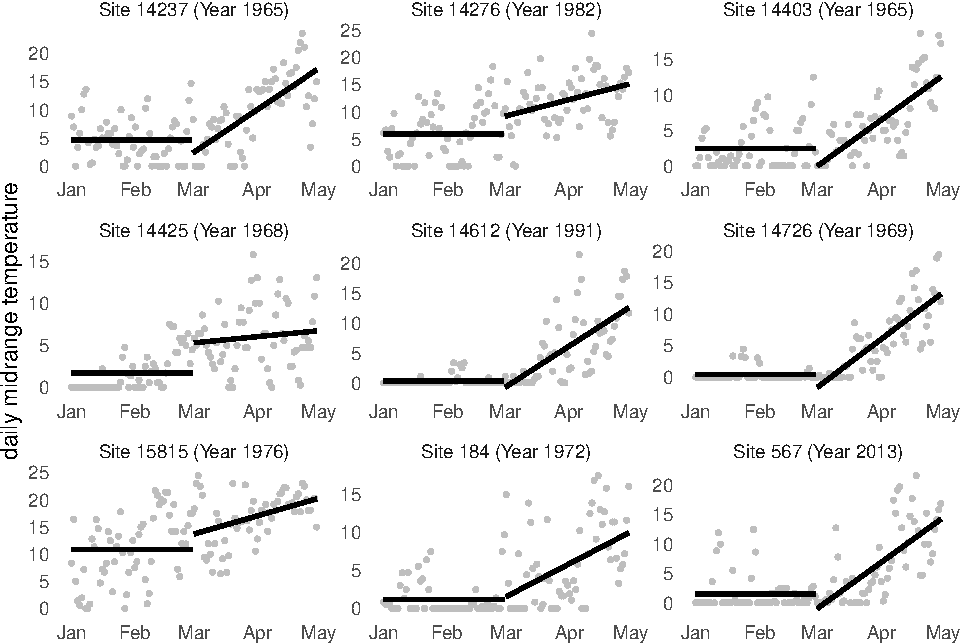
\includegraphics[keepaspectratio]{desynchronization_files/figure-latex/temp_plots-1.pdf}}
\caption{Springtime daily midrange temperatures (points) with \(\alpha\)
(mean from Jan to Feb) and \(\beta\) (slope from Mar to Apr) for nine
randomly selected sites from lilac-honeysuckle dataset (Rosemartin et al. 2015) as measured by 
GHCND stations nearby. Temperatures below 0 are set to 0.}
\end{figure*}

\vfill

\begin{figure*}
\centering
\pandocbounded{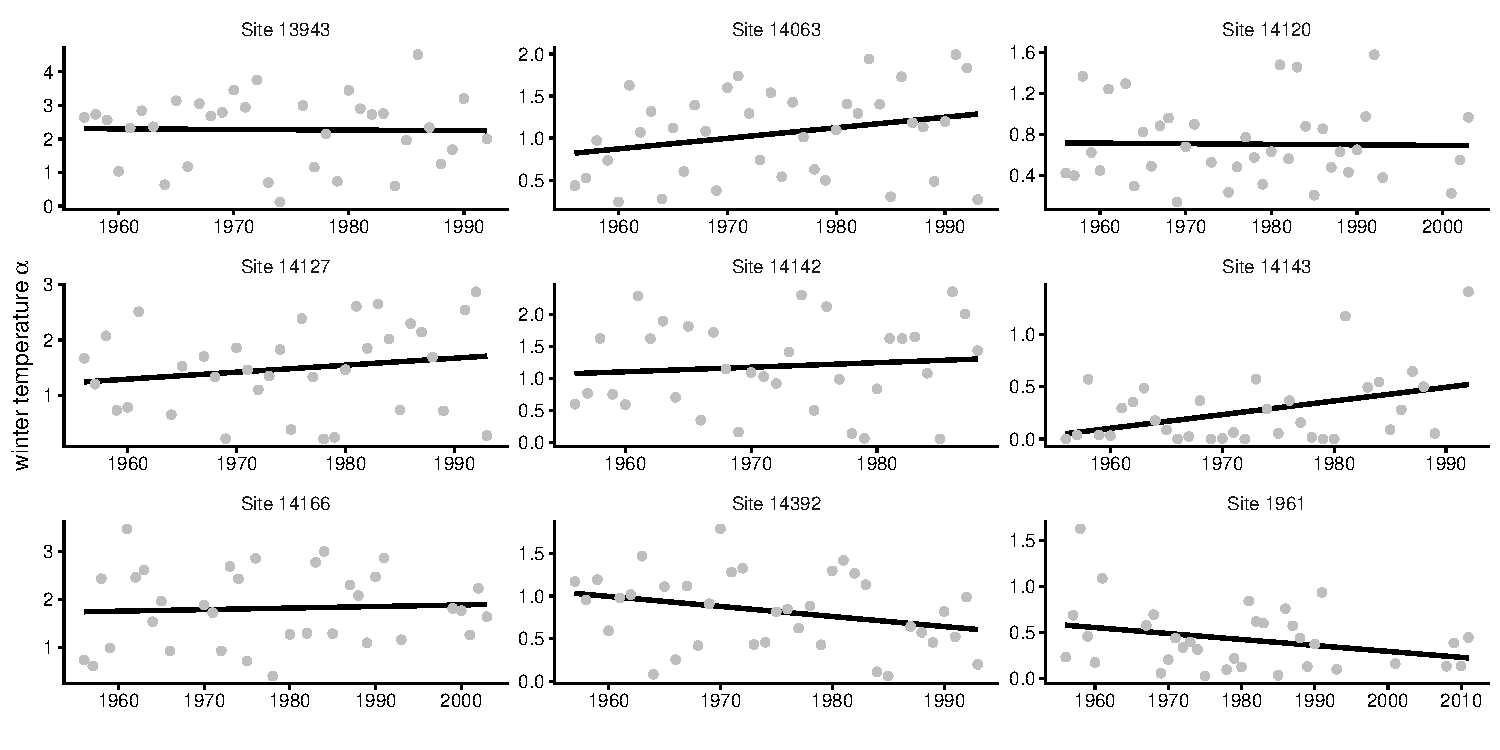
\includegraphics[keepaspectratio]{desynchronization_files/figure-latex/alpha_plots-1.pdf}}
\caption{Changes in \(\alpha\) for the nine sites from lilac-honeysuckle data (Rosemartin et al. 2015) with 
longest running records as as measured by GHCND stations nearby. Trend line and confidence interval calculated using linear regression.}
\end{figure*}

\begin{figure*}
\centering
\pandocbounded{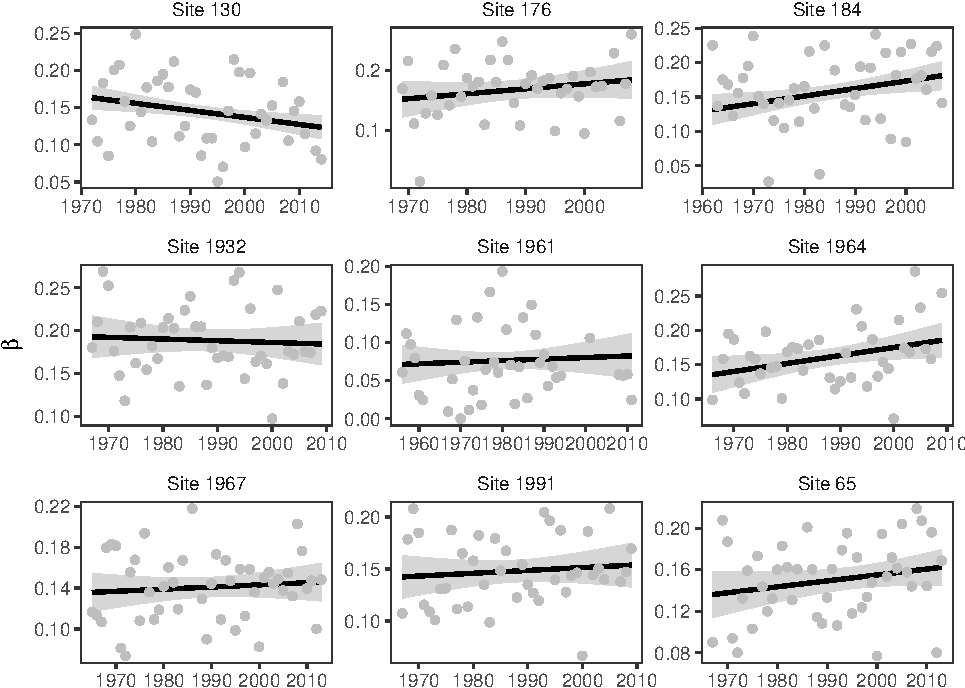
\includegraphics[keepaspectratio]{desynchronization_files/figure-latex/beta_plots-1.pdf}}
\caption{Changes in \(\beta\) for the nine sites from lilac-honeysuckle data (Rosemartin et al. 2015) with 
longest running records as as measured by GHCND stations nearby.  Trend line and confidence interval calculated using linear regression.}
\end{figure*}

\newpage

\subsection{A.4 Simulations}\label{a.3-simulations}

We run two simulations to verify the interpretation of our findings. The
first checks the asymptotic approximation derived in Section A.1. The second
checks the interpretation of the data in Section A.2.

\subsubsection{Simulation 1}\label{simulation-1}

The first simulation verifies the accuracy of the two asymptotic normal
approximations for the hitting time \[
\nu(\tau)=\min\Big\{n\ge 1:\ \sum_{i=1}^n X_i>\tau\Big\}
\] under the model \[
X_i=\alpha+\beta i+\varepsilon_i,\qquad \varepsilon_i\sim \mathrm{Normal}(0,\sigma^2).
\]

We set \(\sigma=20\) and generate daily temperatures
until the threshold \(\tau\) is reached, recording the corresponding
hitting time \(\nu(\tau)\). We repeat this procedure \(R=10{,}000\) times
for thresholds \(\tau = \{1000,2000\}\), \(\alpha = \{2, 4\}\) and
\(\beta = \{0, 0.1 \}\). When \(\beta = 0\), the simulation matches the
winter temperatures regime (regime 1), and when \(\beta = 0.1\), it matches the spring warming regime (regime 2).

We then compare these simulations with the corresponding theoretical approximation.
When \(\beta=0\), we use the winter temperatures regime approximation \[
\nu(\tau)\ \dot{\sim}\ \mathrm{Normal}\!\left(\frac{\tau}{\alpha},\ \frac{\sigma^2 \tau}{\alpha^3}\right).
\] When \(\beta>0\), we use the spring warming regime approximation \[
\nu(\tau)\ \dot{\sim}\ \mathrm{Normal}\!\left(\sqrt{\frac{2\tau}{\beta}}-\frac{\alpha}{\beta}+\frac12,\ 
\frac{\sigma^2}{\beta^{3/2}\sqrt{2\tau}}\right).
\] For each setting we computed the standardized variable \[
z=\frac{\nu(\tau)-\mu}{\mathrm{sd}}.
\] 

The simulated distribution of \(\nu(\tau)\) is represented in Figure 8
below by the histograms, standardized as described above. 
Overlaid is the standard normal density. Across both regimes, the standardized 
histograms align closely with the \(\mathrm{Normal}(0,1)\) curve, and the agreement improves as \(\tau\)
increases, providing a visual confirmation of the derived asymptotic
distributions.

\begin{figure*}
\centering
\pandocbounded{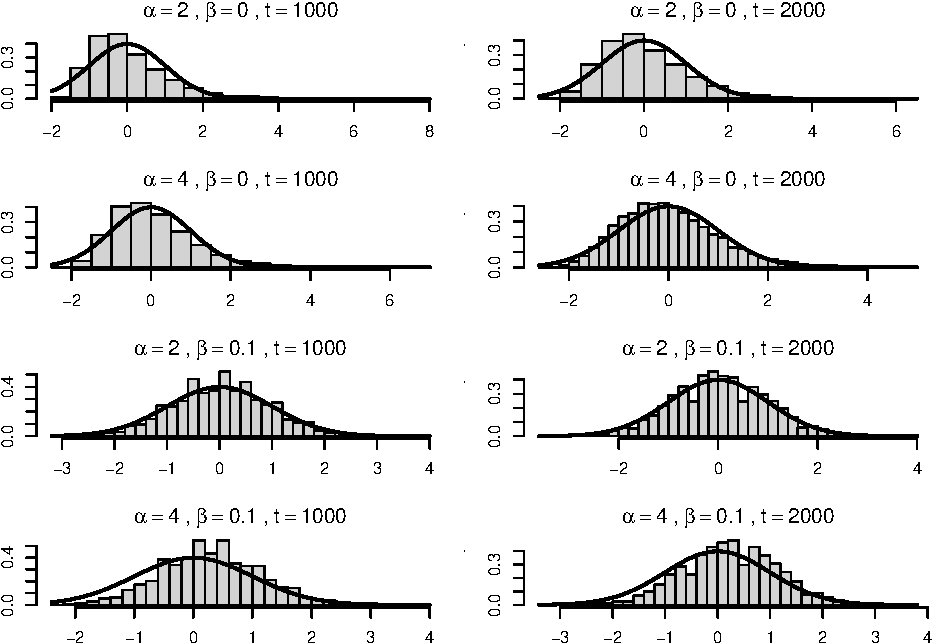
\includegraphics[keepaspectratio]{desynchronization_files/figure-latex/simulation1-1.pdf}}
\caption{Simulations comparing the distribution of bloom dates (histogram) with an asymptotic approximation (solid line) under two regimes: winter temperatures (stationary temperatures, top) and 
spring warming (increasing temperatures, bottom).}
\end{figure*}

\subsubsection{Simulation 2}\label{simulation-2}

To verify our interpretation of the data, we simulate daily temperatures \[
X_i=\mu_i+\varepsilon_i,\qquad \varepsilon_i\sim \mathrm{Normal}(0,\sigma^2),
\] with \(\sigma=20\), where the deterministic component follows \[
\mu_i=
\begin{cases}
\alpha, & i=1,\dots,90 \quad \text{(January--February)},\\[2pt]
\alpha+\beta(i-90), & i=91,\dots,180 \quad \text{(March--April)}.
\end{cases}
\] Bloom occurs when cumulative temperature first exceeds a threshold
\(\tau\), i.e. \[
\nu(\tau)=\min\Big\{n\ge 1:\ \sum_{i=1}^n X_i>\tau\Big\}.
\] We simulated \(R=10{,}000\) independent realizations of \(\nu(\tau)\)
for each combination of \(\alpha\in\{4,8,10\}\),
\(\beta\in\{0.2,0.4,0.8\}\), and \(\tau\in\{1000,2000\}\).
We report the mean (top) and standard deviation (bottom) of \(\nu(\tau)\)
in Tables \ref{tab:sim_mean_1000}-\ref{tab:sim_sd_2000},
arranged with rows indexing \(\alpha\) and columns indexing \(\beta\).

The results reproduce the qualitative patterns observed in the lilac
data. Mean bloom dates decrease as either
\(\alpha\) increases or \(\beta\) increases
(Tables \ref{tab:sim_mean_1000} and
\ref{tab:sim_mean_2000}). Within a fixed \(\alpha\) row, increasing
\(\beta\) reduces the standard deviation of bloom dates
(Tables \ref{tab:sim_sd_1000} and
\ref{tab:sim_sd_2000}), consistent with the prediction that
increasing average temperatures diminish the influence of noise on the
threshold-crossing time. Holding \(\beta\) fixed, the standard deviation is often
larger at higher \(\alpha\) (particularly for \(\beta\in\{0.4,0.8\}\)),
consistent with the prediction that earlier crossings
occur in a flatter portion of the seasonal cycle where microclimate
variability has greater influence.

\begin{table*}[t]
\centering
\caption{Simulated mean and standard deviation of the bloom date
$\nu(t)$ across $R=10{,}000$ replicates with thresholds $\tau\in\{1000,2000\}$. Rows index the winter
level $\alpha$ and columns index the spring warming rate $\beta$.}
\label{tab:sim_piecewise_all}

\setlength{\tabcolsep}{6pt}
\renewcommand{\arraystretch}{1.15}

\begin{minipage}{0.49\linewidth}
\centering
\subcaption{mean, $\tau=1000$}
\label{tab:sim_mean_1000}
\begin{tabular}{lrrr}
\toprule
$\alpha$ $\backslash$ $\beta$ & 0.2 & 0.4 & 0.8 \\
\midrule
4  & 151.66 & 136.83 & 124.86 \\
8  & 114.87 & 111.27 & 106.85 \\
10 &  98.45 &  97.20 &  95.72 \\
\bottomrule
\end{tabular}

\vspace{1.0em}

\subcaption{sd, $\tau=1000$}
\label{tab:sim_sd_1000}
\begin{tabular}{lrrr}
\toprule
$\alpha$ $\backslash$ $\beta$ & 0.2 & 0.4 & 0.8 \\
\midrule
4  & 15.48 & 10.42 &  7.21 \\
8  & 16.53 & 13.27 & 10.50 \\
10 & 15.94 & 14.45 & 12.71 \\
\bottomrule
\end{tabular}
\end{minipage}
\hfill
\begin{minipage}{0.49\linewidth}
\centering
\subcaption{mean, $\tau=2000$}
\label{tab:sim_mean_2000}
\begin{tabular}{lrrr}
\toprule
$\alpha$ $\backslash$ $\beta$ & 0.2 & 0.4 & 0.8 \\
\midrule
4  & 199.54 & 171.15 & 149.16 \\
8  & 169.81 & 152.43 & 137.37 \\
10 & 156.22 & 143.40 & 131.34 \\
\bottomrule
\end{tabular}

\vspace{1.0em}

\subcaption{sd, $\tau=2000$}
\label{tab:sim_sd_2000}
\begin{tabular}{lrrr}
\toprule
$\alpha$ $\backslash$ $\beta$ & 0.2 & 0.4 & 0.8 \\
\midrule
4  & 10.96 & 7.22 & 4.84 \\
8  & 10.93 & 7.50 & 5.11 \\
10 & 10.69 & 7.66 & 5.36 \\
\bottomrule
\end{tabular}
\end{minipage}
\end{table*}

\end{document}
